\chapter{Introducción} \label{chap:1}

\vspace*{5mm}

\section{Motivación personal} \label{sec:1.1}

Desde que empecé mis estudios en Ingeniería Informática tenía bastante claro lo que quería para mi futuro profesional, desarrollar software en la mejor empresa utilizando las últimas tecnologías, y que además lo usara todo el mundo. ¡Qué ingenuo era por aquellos entonces!, aunque por desgracia lo sigo siendo en muchos aspectos. Conforme el transcurso de las asignaturas uno ampliaba su conocimiento, y se daba cuenta de que lo comúnmente llamado \emph{la informática} no consistía solamente en crear software, y que además, todo este campo se basaba en lo que llamaban \emph{ciencias de la computación}. Este campo, a priori no tan amplio, era un obstáculo para mis objetivos. Una desgracia por aquellos entonces, y otra ahora por haber pensado así.

Al mismo tiempo que ampliaba mis conocimientos también ampliaba, sin saberlo, mi red de contactos y escuchaba a profesores y alumnos de último año hablar de sus trabajos. Estos no estaban creando una aplicación para quedar con sus amigos o ver en qué bar se come más barato, hablaban de encontrar el camino más corto en una red de comercio (figura~\ref{fig:1.1}), de minimizar el desperdicio de tela en confección o de predecir apuestas deportivas, ¡las cosas más interesantes que había oído jamás!. Al buscar sobre esos temas descubrí que en la base de todo estaban aquellas ciencias de la computación, así que no podrían ser tan inútiles como pensaba.

\begin{figure}[ht]
    \centering
    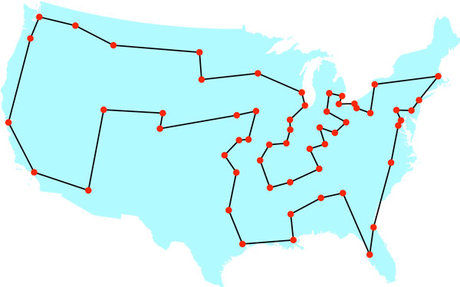
\includegraphics[width=80mm]{figures/ch_01/tsp.jpg}
    \caption{Representación gráfica del problema del viajante de comercio, donde este debe recorrer toda una lista de ciudades minimizando la distancia recorrida. \cite{isherwood2012life}}
    \label{fig:1.1}
\end{figure}

El gran salto vino cuando un grupo de compañeros y yo le pedimos a un profesor, Carlos Antonio García Vallejo, ser sus alumnos internos. Carlos trabajaba en \emph{Aprendizaje Automático}, lo que se conoce in inglés como \emph{Machine Learning}, ¡un campo que era capaz de predecir el futuro!, desde el estado de pacientes, a la bolsa, pasando por el comportamiento humano. Por supuesto que tenía claro que aquello no era una bola de cristal que siempre acertara, y que además, hacer que funcionara bien era de todo menos fácil.

Entonces supe que no tenía nada claro mi futuro profesional, incluso podría convertirse en un futuro académico, pero que intentaría abrazar las ciencias de la computación para ello. Así que de nuevo, agradezco Carlos el haberme abierto la primera puerta en el machine learning, y también a Fernando Sancho Caparrini, mi director de proyecto, por abrirme muchas más, incluso fuera del aprendizaje automático.

\section{Descripción} \label{sec:1.2}

La naturaleza teórica y práctica del machine learning hace que sea un campo en el que se tarde años en poder dominarlo competentemente, por eso una vez acabado este proyecto tan sólo me habré asomado a la inmensidad. Esto no significa que quiera solamente asomarme, tras haberlo hecho estoy ansioso por continuar.

Para que esto ocurriese, he aplicado un método que he refinado a lo largo de los años conviviendo conmigo mismo: acercarme primero desde la práctica\footnote{De ahí el título de este texto, además de ser una referencia al gran libro de [\citeauthor{russell2003artificial}].} para llegar a vislumbrar, aunque levemente, lo que se puede lograr con lo estudiado, y si estoy satisfecho con el resultado, empezar a estudiar la teoría compleja que hay detrás para obtener una mayor comprensión de todo el proceso. Para conseguirlo me he servido básicamente de dos libros, además de diversos artículos y publicaciones online anotadas en la bibliografía. Lo mencionados libros son:

\begin{description}
\item[\emph{Building Machine Learning Systems with Python}] \textbf{[\citeauthor{richert2013building}, ~\citeyear{richert2013building}]} Publicación donde, a través del uso de \emph{Python} como lenguaje de programación, se pone en práctica lo visto en una teoría básicamente explicada.

\item[\emph{Learning From Data: A Short Course}] \textbf{[\citeauthor{abu2012learning}, ~\citeyear{abu2012learning}]} Texto con un gran componente teórico donde se explican conceptos medianamente avanzados de forma sencilla. Un perfecto compañero del libro anterior.
\end{description}

\begin{figure}[ht]
  \centering
  \begin{subfigure}[b]{0.35\textwidth}
    \centering
    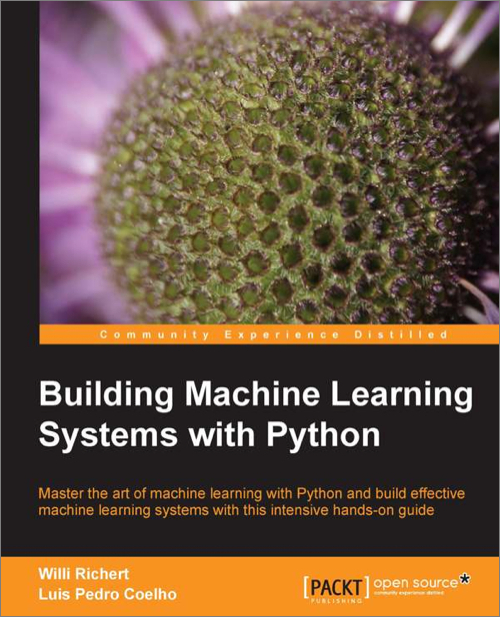
\includegraphics[width=\textwidth]{figures/ch_01/richert2013building.jpg}
    \vspace{10pt}
    \caption{[\citeauthor{richert2013building},~\citeyear{richert2013building}]}
    \label{fig:1.2.a}
  \end{subfigure}
  \hspace{20mm}
  \begin{subfigure}[b]{0.35\textwidth}
    \centering
    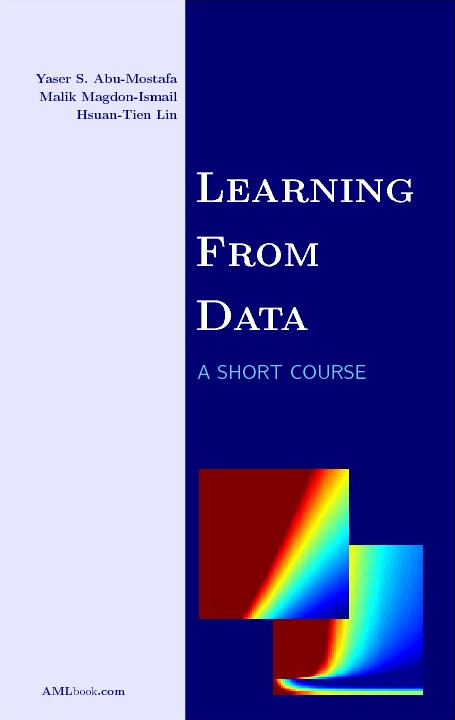
\includegraphics[width=\textwidth]{figures/ch_01/abu2012learning.jpg}
    \caption{[\citeauthor{abu2012learning},~\citeyear{abu2012learning}]}
    \label{fig:1.2.b}
  \end{subfigure}
  \caption{Portadas de los dos libros principales usados durante el proyecto.}
  \label{fig:1.2}
\end{figure}

\section{Objetivos} \label{sec:1.3}

La realización de este proyecto tenía como meta cumplir tres objetivos, los cuales se han cumplido satisfactoriamente:

\begin{itemize}
\item[\textbullet] Aproximarse al estado del arte del machine learning desde un punto de visto pragmático.

\item[\textbullet] Crear una herramienta muy versátil en la que se pueda utilizar machine learning de manera rápida sin lidiar con grandes problemas de instalación.

\item[\textbullet] Aplicar los conocimientos aprendidos y usar la herramienta creada en un caso práctico.
\end{itemize}

\section{Estructura de la memoria} \label{sec:1.4}

Esta memoria se divide en los siguientes capítulos, presentando tres grandes partes:

\begin{description}
\item[\nameref{chap:1}] El presente capítulo.

\large
\item[Parte I] Fundamentos teóricos
\normalsize

\begin{description}
\item[\nameref{chap:2}] Primer capítulo \\ de la teoría, donde se ven distintas definiciones y se estudian cuatro algoritmos muy simples.

\item[\nameref{chap:3}] Segundo y último capítulo de la teoría. Se estudian el resto de algoritmos de la memoria, se ven medidas del rendimiento y una metodología a seguir.
\end{description}

\large
\item[Parte II] Trabajo práctico
\normalsize

\begin{description}
\item[\nameref{chap:4}] En este capítulo se muestra la problemática para crear una herramienta dada la gran cantidad de software a nuestra disposición.

\item[\nameref{chap:5}] Capitulo donde se trata un estudio práctico de principio a fin con un dataset muy interesante y peculiar.
\end{description}

\item[\nameref{chap:6}] Aquí se exponen las conclusiones obtenidas durante el desarrollo del proyecto. Además se comentan los siguientes pasos para el estudio de machine learning y el futuro que tiene este área en diferentes ámbitos.

\pagebreak

\large
\item[Parte III] Apéndices
\normalsize

\begin{description}
\item[\nameref{chap:ap_a}] Apéndice donde se exhibe la documentación disponible en GitHub de la herramienta desarrollada en el capítulo~\ref{chap:4}.

\item[\nameref{chap:ap_b}] Se detalla \\ la documentación expuesta en GitHub del caso práctico desarrollado en el capítulo~\ref{chap:5}.

\item[\nameref{chap:ap_c}] Para finalizar se ofrece la localización en GitHub de los archivos fuente, la versión PDF y la referencia de esta memoria.
\end{description}
\end{description}
